\documentclass[tikz,border=4pt]{standalone}
\usepackage[T1]{fontenc}
\usepackage{lmodern}
\usepackage{amsmath}
\usepackage{pgfplots}
\usetikzlibrary{calc,plotmarks}
\pgfplotsset{compat=1.18}
\definecolor{abmBlue}{HTML}{0072B2}
\definecolor{abmOrange}{HTML}{D55E00}
\definecolor{abmGray}{HTML}{787878}
\definecolor{abmGrid}{HTML}{E7E9EC}
\definecolor{abmShade}{HTML}{F7F8FA}
\pgfplotsset{readable axis/.style={
  width=3.55cm,height=8.2cm,scale only axis,
  xmin=0,xmax=1,ymin=-0.6,ymax=18.8,
  xtick={0,0.25,0.5,0.75,1},xticklabels={0,0.25,0.5,0.75,1},
  ytick=\empty,axis x line*=bottom,axis y line=none,
  axis line style={black!65,line width=0.45pt},
  tick align=outside,tick style={black!65,line width=0.4pt},
  tick label style={font=\fontsize{7.5}{9}\selectfont},
  xmajorgrids=true,ymajorgrids=false,grid style={abmGrid,line width=0.35pt},
  xlabel={PAWN index},xlabel style={font=\fontsize{8}{10}\selectfont},
  clip=false
}}
% Use full-precision endpoints as arguments; rounding affects labels only.
\newcommand{\MCnumber}[1]{\pgfmathprintnumber[fixed,fixed zerofill,precision=3]{#1}}
\begin{document}
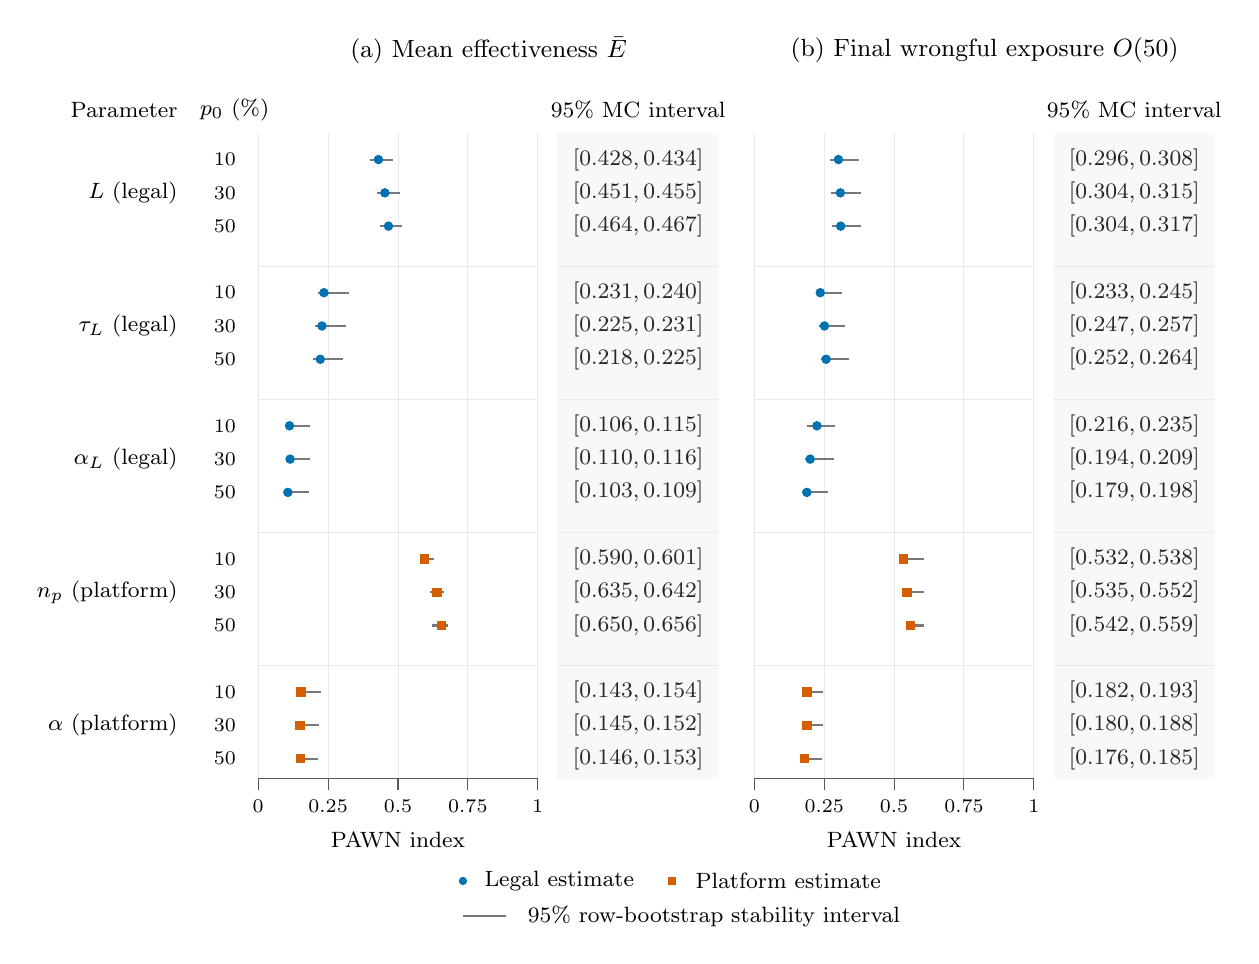
\begin{tikzpicture}
\begin{axis}[readable axis,name=main0,at={(0.00cm,0cm)},anchor=south west]
% Each parameter group contains p0 = 10, 30, 50 percent from top to bottom.
\draw[abmGrid,line width=0.35pt] (axis cs:0,14.8) -- (axis cs:1,14.8);
\draw[abmGrid,line width=0.35pt] (axis cs:0,10.8) -- (axis cs:1,10.8);
\draw[abmGrid,line width=0.35pt] (axis cs:0,6.8) -- (axis cs:1,6.8);
\draw[abmGrid,line width=0.35pt] (axis cs:0,2.8) -- (axis cs:1,2.8);
\addplot[abmGray,line width=0.75pt,unbounded coords=jump,forget plot] coordinates {
(0.398908568972,18) (0.483669117647,18) (nan,nan)
(0.423596750585,17) (0.506005060034,17) (nan,nan)
(0.434057026144,16) (0.515538022942,16) (nan,nan)
(0.213303156888,14) (0.325980803983,14) (nan,nan)
(0.203054638219,13) (0.314578724054,13) (nan,nan)
(0.195982727889,12) (0.301571484726,12) (nan,nan)
(0.116220761019,10) (0.186960714449,10) (nan,nan)
(0.118867078393,9) (0.185645778307,9) (nan,nan)
(0.117566892432,8) (0.182860163087,8) (nan,nan)
};
\addplot[only marks,mark=*,mark size=1.5pt,abmBlue,forget plot] coordinates {
(0.43,18)
(0.453,17)
(0.466,16)
(0.235,14)
(0.228,13)
(0.222,12)
(0.112,10)
(0.114,9)
(0.106,8)
};
\addplot[abmGray,line width=0.75pt,unbounded coords=jump,forget plot] coordinates {
(0.580985606061,6) (0.628801020408,6) (nan,nan)
(0.613374667553,5) (0.665,5) (nan,nan)
(0.622510689609,4) (0.678014583333,4) (nan,nan)
(0.150751575017,2) (0.224259691544,2) (nan,nan)
(0.147838689622,1) (0.217089946826,1) (nan,nan)
(0.145527635586,0) (0.212084027778,0) (nan,nan)
};
\addplot[only marks,mark=square*,mark size=1.5pt,abmOrange,forget plot] coordinates {
(0.595,6)
(0.64,5)
(0.655,4)
(0.153,2)
(0.15,1)
(0.152,0)
};
\node[anchor=east,font=\fontsize{8}{10}\selectfont] at ([xshift=-0.90cm]axis cs:0,17) {$L$ (legal)};
\node[anchor=east,font=\fontsize{7.5}{9}\selectfont] at ([xshift=-0.16cm]axis cs:0,18) {10};
\node[anchor=east,font=\fontsize{7.5}{9}\selectfont] at ([xshift=-0.16cm]axis cs:0,17) {30};
\node[anchor=east,font=\fontsize{7.5}{9}\selectfont] at ([xshift=-0.16cm]axis cs:0,16) {50};
\node[anchor=east,font=\fontsize{8}{10}\selectfont] at ([xshift=-0.90cm]axis cs:0,13) {$\tau_L$ (legal)};
\node[anchor=east,font=\fontsize{7.5}{9}\selectfont] at ([xshift=-0.16cm]axis cs:0,14) {10};
\node[anchor=east,font=\fontsize{7.5}{9}\selectfont] at ([xshift=-0.16cm]axis cs:0,13) {30};
\node[anchor=east,font=\fontsize{7.5}{9}\selectfont] at ([xshift=-0.16cm]axis cs:0,12) {50};
\node[anchor=east,font=\fontsize{8}{10}\selectfont] at ([xshift=-0.90cm]axis cs:0,9) {$\alpha_L$ (legal)};
\node[anchor=east,font=\fontsize{7.5}{9}\selectfont] at ([xshift=-0.16cm]axis cs:0,10) {10};
\node[anchor=east,font=\fontsize{7.5}{9}\selectfont] at ([xshift=-0.16cm]axis cs:0,9) {30};
\node[anchor=east,font=\fontsize{7.5}{9}\selectfont] at ([xshift=-0.16cm]axis cs:0,8) {50};
\node[anchor=east,font=\fontsize{8}{10}\selectfont] at ([xshift=-0.90cm]axis cs:0,5) {$n_p$ (platform)};
\node[anchor=east,font=\fontsize{7.5}{9}\selectfont] at ([xshift=-0.16cm]axis cs:0,6) {10};
\node[anchor=east,font=\fontsize{7.5}{9}\selectfont] at ([xshift=-0.16cm]axis cs:0,5) {30};
\node[anchor=east,font=\fontsize{7.5}{9}\selectfont] at ([xshift=-0.16cm]axis cs:0,4) {50};
\node[anchor=east,font=\fontsize{8}{10}\selectfont] at ([xshift=-0.90cm]axis cs:0,1) {$\alpha$ (platform)};
\node[anchor=east,font=\fontsize{7.5}{9}\selectfont] at ([xshift=-0.16cm]axis cs:0,2) {10};
\node[anchor=east,font=\fontsize{7.5}{9}\selectfont] at ([xshift=-0.16cm]axis cs:0,1) {30};
\node[anchor=east,font=\fontsize{7.5}{9}\selectfont] at ([xshift=-0.16cm]axis cs:0,0) {50};
\node[anchor=east,font=\fontsize{8}{10}\selectfont] at ([xshift=-0.90cm]axis cs:0,19.5) {Parameter};
\node[anchor=center,font=\fontsize{8}{10}\selectfont] at ([xshift=-0.30cm]axis cs:0,19.5) {$p_0$ (\%)};
\path[fill=abmShade] ([xshift=0.25cm]axis cs:1,-0.6) rectangle ([xshift=2.30cm]axis cs:1,18.8);
\draw[abmGrid,line width=0.35pt] ([xshift=0.25cm]axis cs:1,14.8) -- ([xshift=2.30cm]axis cs:1,14.8);
\draw[abmGrid,line width=0.35pt] ([xshift=0.25cm]axis cs:1,10.8) -- ([xshift=2.30cm]axis cs:1,10.8);
\draw[abmGrid,line width=0.35pt] ([xshift=0.25cm]axis cs:1,6.8) -- ([xshift=2.30cm]axis cs:1,6.8);
\draw[abmGrid,line width=0.35pt] ([xshift=0.25cm]axis cs:1,2.8) -- ([xshift=2.30cm]axis cs:1,2.8);
\node[font=\fontsize{8}{10}\selectfont,text=black!85] at ([xshift=1.275cm]axis cs:1,18) {[\MCnumber{0.428},\,\MCnumber{0.434}]};
\node[font=\fontsize{8}{10}\selectfont,text=black!85] at ([xshift=1.275cm]axis cs:1,17) {[\MCnumber{0.451},\,\MCnumber{0.455}]};
\node[font=\fontsize{8}{10}\selectfont,text=black!85] at ([xshift=1.275cm]axis cs:1,16) {[\MCnumber{0.464},\,\MCnumber{0.467}]};
\node[font=\fontsize{8}{10}\selectfont,text=black!85] at ([xshift=1.275cm]axis cs:1,14) {[\MCnumber{0.231},\,\MCnumber{0.24}]};
\node[font=\fontsize{8}{10}\selectfont,text=black!85] at ([xshift=1.275cm]axis cs:1,13) {[\MCnumber{0.225},\,\MCnumber{0.231}]};
\node[font=\fontsize{8}{10}\selectfont,text=black!85] at ([xshift=1.275cm]axis cs:1,12) {[\MCnumber{0.218},\,\MCnumber{0.225}]};
\node[font=\fontsize{8}{10}\selectfont,text=black!85] at ([xshift=1.275cm]axis cs:1,10) {[\MCnumber{0.106},\,\MCnumber{0.115}]};
\node[font=\fontsize{8}{10}\selectfont,text=black!85] at ([xshift=1.275cm]axis cs:1,9) {[\MCnumber{0.11},\,\MCnumber{0.116}]};
\node[font=\fontsize{8}{10}\selectfont,text=black!85] at ([xshift=1.275cm]axis cs:1,8) {[\MCnumber{0.103},\,\MCnumber{0.109}]};
\node[font=\fontsize{8}{10}\selectfont,text=black!85] at ([xshift=1.275cm]axis cs:1,6) {[\MCnumber{0.59},\,\MCnumber{0.601025}]};
\node[font=\fontsize{8}{10}\selectfont,text=black!85] at ([xshift=1.275cm]axis cs:1,5) {[\MCnumber{0.635},\,\MCnumber{0.642}]};
\node[font=\fontsize{8}{10}\selectfont,text=black!85] at ([xshift=1.275cm]axis cs:1,4) {[\MCnumber{0.65},\,\MCnumber{0.656}]};
\node[font=\fontsize{8}{10}\selectfont,text=black!85] at ([xshift=1.275cm]axis cs:1,2) {[\MCnumber{0.143},\,\MCnumber{0.154}]};
\node[font=\fontsize{8}{10}\selectfont,text=black!85] at ([xshift=1.275cm]axis cs:1,1) {[\MCnumber{0.145},\,\MCnumber{0.152}]};
\node[font=\fontsize{8}{10}\selectfont,text=black!85] at ([xshift=1.275cm]axis cs:1,0) {[\MCnumber{0.146},\,\MCnumber{0.153}]};
\node[align=center,font=\fontsize{8}{10}\selectfont] at ([xshift=1.275cm]axis cs:1,19.5) {95\% MC interval};
\end{axis}
\begin{axis}[readable axis,name=main1,at={(6.30cm,0cm)},anchor=south west]
% Each parameter group contains p0 = 10, 30, 50 percent from top to bottom.
\draw[abmGrid,line width=0.35pt] (axis cs:0,14.8) -- (axis cs:1,14.8);
\draw[abmGrid,line width=0.35pt] (axis cs:0,10.8) -- (axis cs:1,10.8);
\draw[abmGrid,line width=0.35pt] (axis cs:0,6.8) -- (axis cs:1,6.8);
\draw[abmGrid,line width=0.35pt] (axis cs:0,2.8) -- (axis cs:1,2.8);
\addplot[abmGray,line width=0.75pt,unbounded coords=jump,forget plot] coordinates {
(0.269694233507,18) (0.37550545393,18) (nan,nan)
(0.272994281046,17) (0.380839870582,17) (nan,nan)
(0.27895549062,16) (0.380837176974,16) (nan,nan)
(0.219367857143,14) (0.314996127682,14) (nan,nan)
(0.230063207058,13) (0.324470952911,13) (nan,nan)
(0.239517752973,12) (0.33791507454,12) (nan,nan)
(0.187664355647,10) (0.290069801092,10) (nan,nan)
(0.180864834115,9) (0.283362712337,9) (nan,nan)
(0.170038091081,8) (0.262666471114,8) (nan,nan)
};
\addplot[only marks,mark=*,mark size=1.5pt,abmBlue,forget plot] coordinates {
(0.301,18)
(0.308,17)
(0.309,16)
(0.236,14)
(0.251,13)
(0.257,12)
(0.224,10)
(0.2,9)
(0.188,8)
};
\addplot[abmGray,line width=0.75pt,unbounded coords=jump,forget plot] coordinates {
(0.524395068869,6) (0.606891650212,6) (nan,nan)
(0.532786737401,5) (0.60773738354,5) (nan,nan)
(0.542978296146,4) (0.608607295646,4) (nan,nan)
(0.174553703704,2) (0.245078434635,2) (nan,nan)
(0.171852203647,1) (0.244363687783,1) (nan,nan)
(0.171479237288,0) (0.240927460339,0) (nan,nan)
};
\addplot[only marks,mark=square*,mark size=1.5pt,abmOrange,forget plot] coordinates {
(0.533,6)
(0.547,5)
(0.559,4)
(0.189,2)
(0.188,1)
(0.179,0)
};
\path[fill=abmShade] ([xshift=0.25cm]axis cs:1,-0.6) rectangle ([xshift=2.30cm]axis cs:1,18.8);
\draw[abmGrid,line width=0.35pt] ([xshift=0.25cm]axis cs:1,14.8) -- ([xshift=2.30cm]axis cs:1,14.8);
\draw[abmGrid,line width=0.35pt] ([xshift=0.25cm]axis cs:1,10.8) -- ([xshift=2.30cm]axis cs:1,10.8);
\draw[abmGrid,line width=0.35pt] ([xshift=0.25cm]axis cs:1,6.8) -- ([xshift=2.30cm]axis cs:1,6.8);
\draw[abmGrid,line width=0.35pt] ([xshift=0.25cm]axis cs:1,2.8) -- ([xshift=2.30cm]axis cs:1,2.8);
\node[font=\fontsize{8}{10}\selectfont,text=black!85] at ([xshift=1.275cm]axis cs:1,18) {[\MCnumber{0.296},\,\MCnumber{0.308}]};
\node[font=\fontsize{8}{10}\selectfont,text=black!85] at ([xshift=1.275cm]axis cs:1,17) {[\MCnumber{0.304},\,\MCnumber{0.315}]};
\node[font=\fontsize{8}{10}\selectfont,text=black!85] at ([xshift=1.275cm]axis cs:1,16) {[\MCnumber{0.304},\,\MCnumber{0.317}]};
\node[font=\fontsize{8}{10}\selectfont,text=black!85] at ([xshift=1.275cm]axis cs:1,14) {[\MCnumber{0.233},\,\MCnumber{0.245}]};
\node[font=\fontsize{8}{10}\selectfont,text=black!85] at ([xshift=1.275cm]axis cs:1,13) {[\MCnumber{0.247},\,\MCnumber{0.257}]};
\node[font=\fontsize{8}{10}\selectfont,text=black!85] at ([xshift=1.275cm]axis cs:1,12) {[\MCnumber{0.252},\,\MCnumber{0.264}]};
\node[font=\fontsize{8}{10}\selectfont,text=black!85] at ([xshift=1.275cm]axis cs:1,10) {[\MCnumber{0.216},\,\MCnumber{0.235}]};
\node[font=\fontsize{8}{10}\selectfont,text=black!85] at ([xshift=1.275cm]axis cs:1,9) {[\MCnumber{0.194},\,\MCnumber{0.209}]};
\node[font=\fontsize{8}{10}\selectfont,text=black!85] at ([xshift=1.275cm]axis cs:1,8) {[\MCnumber{0.179},\,\MCnumber{0.198}]};
\node[font=\fontsize{8}{10}\selectfont,text=black!85] at ([xshift=1.275cm]axis cs:1,6) {[\MCnumber{0.532},\,\MCnumber{0.538}]};
\node[font=\fontsize{8}{10}\selectfont,text=black!85] at ([xshift=1.275cm]axis cs:1,5) {[\MCnumber{0.535},\,\MCnumber{0.552}]};
\node[font=\fontsize{8}{10}\selectfont,text=black!85] at ([xshift=1.275cm]axis cs:1,4) {[\MCnumber{0.542},\,\MCnumber{0.559}]};
\node[font=\fontsize{8}{10}\selectfont,text=black!85] at ([xshift=1.275cm]axis cs:1,2) {[\MCnumber{0.182},\,\MCnumber{0.193}]};
\node[font=\fontsize{8}{10}\selectfont,text=black!85] at ([xshift=1.275cm]axis cs:1,1) {[\MCnumber{0.18},\,\MCnumber{0.188}]};
\node[font=\fontsize{8}{10}\selectfont,text=black!85] at ([xshift=1.275cm]axis cs:1,0) {[\MCnumber{0.176},\,\MCnumber{0.185}]};
\node[align=center,font=\fontsize{8}{10}\selectfont] at ([xshift=1.275cm]axis cs:1,19.5) {95\% MC interval};
\end{axis}
\node[font=\fontsize{9}{11}\selectfont] at (2.925,9.25) {(a) Mean effectiveness $\bar E$};
\node[font=\fontsize{9}{11}\selectfont] at (9.225,9.25) {(b) Final wrongful exposure $O(50)$};
\begin{scope}[shift={(5.2,-1.3)} ]

\fill[abmBlue] (-2.6,0) circle[radius=1.5pt];
\node[anchor=west,font=\fontsize{8}{10}\selectfont] at (-2.45,0) {Legal estimate};
\fill[abmOrange] (0.00,-0.053) rectangle (0.106,0.053);
\node[anchor=west,font=\fontsize{8}{10}\selectfont] at (0.23,0) {Platform estimate};
\draw[abmGray,line width=0.75pt] (-2.6,-0.45) -- (-2.05,-0.45);
\node[anchor=west,font=\fontsize{8}{10}\selectfont] at (-1.90,-0.45) {95\% row-bootstrap stability interval};
\end{scope}
\end{tikzpicture}
\end{document}
